\documentclass[11pt]{article}
\usepackage{amsmath,amssymb,amsthm}
\usepackage[utf8]{inputenc}
\usepackage{graphicx}
\usepackage{xcolor}

\DeclareMathOperator*{\E}{\mathbb{E}}
\let\Pr\relax
\DeclareMathOperator*{\Pr}{\mathbb{P}}

\newcommand{\eps}{\varepsilon}
\newcommand{\inprod}[1]{\left\langle #1 \right\rangle}
\newcommand{\R}{\mathbb{R}}

\theoremstyle{definition} \newtheorem{Theorem}{theorem}

\newcommand{\handout}[5]{
  \noindent
  \begin{center}
  \framebox{
    \vbox{
      \hbox to 6.38in { \textcolor{black}{\bf CS 134: Networks } \hfill #4  }
      \vspace{1mm}
      \hbox to 6.42in { #3 {\hfill #2 } }
      \vspace{0.0mm}
      \hbox to 6.38in { { \hfill} }
    }
  }
  \end{center}
  \vspace*{0mm}
}

\newcommand{\pset}[3]{\handout{{#1}}{\textcolor{red}{Due: #2}}{\textcolor{black}{#3}}{\textcolor{gray}{\textbf{Problem set #1}}}}

\newtheorem{theorem}{Theorem}
\newtheorem{corollary}[theorem]{Corollary}
\newtheorem{lemma}[theorem]{Lemma}
\newtheorem{observation}[theorem]{Observation}
\newtheorem{proposition}[theorem]{Proposition}
\newtheorem{definition}[theorem]{Definition}
\newtheorem{claim}[theorem]{Claim}
\newtheorem{fact}[theorem]{Fact}
\newtheorem{assumption}[theorem]{Assumption}
\newtheorem{remark}[theorem]{Remark}

\newtheorem*{theorem*}{Theorem}
\newtheorem*{notation*}{Notation}
\newtheorem*{assumption*}{Assumption}
\newtheorem*{fact*}{Fact}
\newtheorem*{claim*}{Claim}
\newtheorem*{definition*}{Definition}
\newtheorem*{exercise*}{Exercise}
\newtheorem*{lemma*}{Lemma}
\newtheorem*{remark*}{Remark}

% 1-inch margins, from fullpage.sty by H.Partl, Version 2, Dec. 15, 1988.
\topmargin 0pt
\advance \topmargin by -\headheight
\advance \topmargin by -\headsep
\textheight 8.9in
\oddsidemargin 0pt
\evensidemargin \oddsidemargin
\marginparwidth 0.5in
\textwidth 6.5in

\parindent 0in
\parskip 1.5ex


\usepackage[margin=.9in]{geometry}
\usepackage{amsmath}
\usepackage{tikz}
\usepackage{float}
\usepackage{filecontents}
\usepackage{pgfplots, pgfplotstable}
\usepackage{listings}

%\usepgfplotslibrary{statistics}
\usepackage[T1]{fontenc}
%\usepackage{enumitem}
\usepackage{hyperref}
\usetikzlibrary{calc,intersections,through,backgrounds,shadings}
\usetikzlibrary{shapes.geometric}
\usetikzlibrary{through}

\usepackage[nofiglist,nomarkers]{endfloat}
\renewcommand{\efloatseparator}{\mbox{}}

\usepackage{exercise}
\renewcommand{\ExerciseHeader}{{ \textbf{
\ExerciseName \ \ExerciseHeaderNB \ExerciseHeaderTitle
\ExerciseHeaderOrigin.}}}

\usepackage{pgfplots}
\pgfplotsset{
%  compatgraph=newest,
  xlabel near ticks,
  ylabel near ticks
}



\begin{document}

\pset{1}{\textbf{Noon, Wednesday 2/1/2017}}{{Prof. Yaron Singer}}


\textbf{Resources:} This problem set contains $5$ parts.  All the relevant concepts can be found in the lecture and section notes.  For further reading you may wish to consult Chapter $2$ of Matt Jackson's book. 

\paragraph{1. Diameter and Average Path Length (Jackson 2.2.2). } 
\begin{itemize} 
\item The \emph{distance} between two nodes is the length of a geodesic between them -- i.e. the smallest number of links in the graph needed to connect the two nodes.  For example, the distance between the nodes $b$ and $e$ in network $A$ in the figure at the bottom is $2$. If there is no path between two nodes, we say that the distance between them is infinite. 
\item The \emph{diameter} of a network is the largest distance between any two nodes in the network. 
\item The \emph{average path length} between the nodes of a network is the arithmetic mean of the distances between all pairs of nodes in the network. For example, consider the following network: $$(\{a,b,c\}, \{ab,ac\}).$$ The average path length is: $$ \frac{1}{3} \Big [ \text{distance}(a,b) + \text{distance}(a,c) + \text{distance}(b,c)  \Big ] = \frac{1}{3} \Big [ 1 +2 + 1  \Big] = \frac{4}{3}. $$
\end{itemize}

\begin{enumerate}
\item[\textbf{a.}] What is the distance between nodes $e$ and $i$ in network $B$? 
\item[\textbf{b.}] What is the diameter of the following network? $$(\{a,b,c,d,e\}, \{ ab,ac, ad,de\})$$ 
\item[\textbf{c.}] What is the average path length in the following network?  $$(\{a,b,c,d\}, \{ab,ac, ad\})$$ 
\end{enumerate}




\paragraph{2. Cliquishness, Cohesiveness and Clustering (Jackson 2.2.3). } Note we use the words ``network'' and ``graph'' interchangeably.
\begin{itemize}
\item A \emph{complete subgraph} of a graph is a nonempty subgraph $C$ with every two nodes in $C$ linked. A \emph{clique} of graph $G$ is\footnote{Intuitively, cliques are the biggest completely connected pieces of a network.} a maximal complete subgraph of $G$. In other words, it is a complete subgraph $C$ of $G$ that is not a subgraph of any larger complete subgraph of $G$. For example, $(\{a,c\}, \{ac\})$ is a clique of network $A$ but the following subgraph is not: $$(\{b,d,e,f\}, \{bd,de,df,ef\})$$   

\item[\textbf{a.}] Represent a clique of network $B$ via a picture. 


\item The most common way of measuring the cohesiveness of a network is based on transitive triples (or clustering). The most basic clustering measure is to perform the following exercise. Look at all situations in which two edges emanate from the same node (for example, edges $ij$ and $ik$ both involve node $i$) and ask how often the edge $jk$ is then also in the network. We call this likelihood the \emph{clustering coefficient}. For example, the clustering coefficient of network $A$ is $\frac{3}{5}$. To see this, note that there are five pairs of nodes that are linked to a common node ($bf$, $be$, $ef$, $df$, $de$), and only three of these ($de$, $ef$, $df$) are themselves linked. In a friendship network, the clustering coefficient  tells us how likely it is that two individuals with a common friend are friends themselves.\footnote{Another measure often used is the  \emph{average clustering coefficient}. To compute that, we look at each node $i$ and compute $i$'s clustering coefficient $c_i$---defined as the clustering coefficient of the subgraph consisting of $i$, its neighbors, and all links among them in the original graph. Then take the arithmetic mean of $c_i$ across nodes. See Jackson for details.}  
\item [\textbf{b.}] Compute the clustering coefficient of network $B$. 
\end{itemize}

\paragraph{3. Graph Cuts and Expansion.} 
\begin{itemize}
\item Given a graph $G=(V,E)$, and two disjoint subsets of nodes $S,T \subset V$ with $S \cap T = \emptyset$, a \emph{cut} $C(S,T)$ is the set of all edges that have one end point in $S$ and another endpoint in $T$.  For example, if we have a graph $G=(V,E)$ with set of nodes $\{u,v,w,x,y,z\}$ and the set of edges $\{uw, ux, vx, vz, wx, xy, yz \}$, for
$S = {u,v}$ and $T={w,x,y}$ the cut is $C(S,T) = \{uw,ux,vx\}$. 

\item The \emph{expansion} of a graph $G = (V,E)$ is the minimum, over all cuts we can make of the number of edges crossing the cut divided by the number of vertices in the smaller half of the cut. Formally:
 \[ \min_{S \subseteq V} \frac{|C(S,V\setminus S)|}{\min\{|S|,|V\setminus S|\}}.\]
%
Show that the expansion of a graph can also be expressed as $\alpha$, where:
 \[ \alpha = \min_{\substack{S \subseteq V, \\1 \leq |S| \leq \frac{n}{2} }} \frac{|e(S)|}{|S|} \]
where $e(S)$ is the number of edges leaving the set $S$.

**Solution: Since rtaehtiauht
\end{itemize}


\paragraph{4. Basics of Erd\H{o}s-R\'{e}nyi: Playing with Small Graphs.}

Consider the set of $n=4$ nodes $V=\{a,b,c,d\}$. Suppose that an edge (i.e., link) between any two nodes $i$ and $j$ forms with probability $p \in (0,1)$, independently of all other edges. This is the $G(n,p)$ Erd\H{o}s-R\'{e}nyi random graph with $n=4$.

\begin{enumerate}

\item[\textbf{a.}] For this graph on $n=4$ nodes, what is the probability that the graph has  (i) no edges, (ii) one edge and (iii) more than one edge? The only variable in your answer should be $p$.

\item[\textbf{b.}] What is the expected degree of each node in $G(4,0.5)$?

\item[\textbf{c.}] Generate a random graph $G(4,0.5)$ on the nodes  $V=\{a,b,c,d\}$ using a coin (as was done in class). Write down your graph (any of the descriptions introduced in Problem Set 1 are okay).

\item[\textbf{d.}] \textbf{Bonus question (not mandatory):} Plot the degree distribution of the graph you just made. Plot on top of it the Poisson distribution (see lecture notes for more information) with $\mu$, the mean, equal to the expected degree you computed in (b). Comment on the quality of the approximation.


\end{enumerate}


\paragraph{5. Compound Growth.} Fix an integer $k \geq 1$ and consider the sequence $s_n \equiv \left[(1+\frac{1}{k})^{k} \right]^n = \left[(1+\frac{1}{k})^k\right]^1, \left[(1+\frac{1}{k})^k\right]^2, \dots$. 
\begin{itemize}
\item[\textbf{a.}] Show that $\left( 1 + \frac{1}{k} \right)^{k} \geq 2$. 
\item[\textbf{b.}]  Show that $n \geq 20$ implies  $\left[(1+\frac{1}{k})^{k} \right]^n \geq 10^6$. 
\item[\textbf{c.}] If you had one dollar to invest, and were guaranteed that you will earn $p$ percent every day on your money, how long would it take you to become a millionaire (if you aren't one already)? 
\end{itemize}


%%%%%%%%%%% Network A
\begin{figure}[t] 
\centering
\caption{Network $A$}
\label{example}
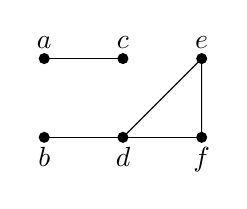
\begin{tikzpicture} [scale=1]

\coordinate [label=above:{$a$}] (a) at (0,1);
\coordinate [label=below:{$b$}] (b) at (0,0);
\coordinate [label=above:{$c$}] (c) at (1,1);
\coordinate [label=below:{$d$}] (d) at (1,0);
\coordinate [label=above:{$e$}] (e) at (2,1);
\coordinate [label=below:{$f$}] (f) at (2,0);

\fill (a) circle (2pt);
\fill (b) circle (2pt);
\fill (c) circle (2pt);
\fill (d) circle (2pt);
\fill (e) circle (2pt);
\fill (f) circle (2pt);

\draw (a)--(c);
\draw (d)--(e)--(f);
\draw (b)--(d)--(f);

\end{tikzpicture}
\end{figure}

%%%%%%%%% Network B
\begin{figure} 
\centering
\caption{Network $B$}
\label{exercise}
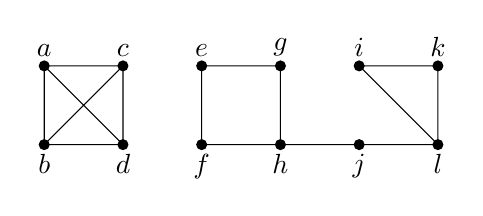
\begin{tikzpicture} [scale=1]

\coordinate [label=above:{$a$}] (a) at (0,1);
\coordinate [label=below:{$b$}] (b) at (0,0);
\coordinate [label=above:{$c$}] (c) at (1,1);
\coordinate [label=below:{$d$}] (d) at (1,0);
\coordinate [label=above:{$e$}] (e) at (2,1);
\coordinate [label=below:{$f$}] (f) at (2,0);
\coordinate [label=above:{$g$}] (g) at (3,1);
\coordinate [label=below:{$h$}] (h) at (3,0);
\coordinate [label=above:{$i$}] (i) at (4,1);
\coordinate [label=below:{$j$}] (j) at (4,0);
\coordinate [label=above:{$k$}] (k) at (5,1);
\coordinate [label=below:{$l$}] (l) at (5,0);

\fill (a) circle (2pt);
\fill (b) circle (2pt);
\fill (c) circle (2pt);
\fill (d) circle (2pt);
\fill (e) circle (2pt);
\fill (f) circle (2pt);
\fill (g) circle (2pt);
\fill (h) circle (2pt);
\fill (i) circle (2pt);
\fill (j) circle (2pt);
\fill (k) circle (2pt);
\fill (l) circle (2pt);

\draw (a)--(d)--(c)--(b)--(a)--(c)--(d)--(b);
\draw (h)--(f)--(e)--(g)--(h)-- (j)--(l)--(k)--(i)--(l);

\end{tikzpicture}
\end{figure}




\end{document}

